% MINA poster -- Columbia Undergraduate Research Symposium 2026
% Build: pdflatex (twice) -- see build.sh.  Page = 41in x 36in landscape.
% Sans = Helvetica (URW, Type1) via helvet: this TeX Live has no luaotfload,
% so lualatex+fontspec is unavailable; helvet embeds cleanly under pdflatex.
\documentclass[final]{beamer}
\usepackage[orientation=landscape,size=custom,width=104.14,height=91.44,scale=1.14]{beamerposter}
\usepackage[T1]{fontenc}
\usepackage{helvet}
\renewcommand{\familydefault}{\sfdefault}
\usepackage{tikz}
\usetikzlibrary{arrows.meta,positioning,calc}
\usepackage[most]{tcolorbox}
\usepackage{graphicx}
\usepackage{ragged2e}

\graphicspath{{figures/}}

% ---------- palette (text/accents; figure colours live in the PDFs) ----------
\definecolor{colBlue}{HTML}{10305F}    % headings / deep navy
\definecolor{colAccent}{HTML}{1F5FAE}  % rules, borders
\definecolor{inkGrey}{HTML}{2B2B2B}    % body text
\definecolor{famTF}{HTML}{1f77b4}
\definecolor{famGPCR}{HTML}{ff7f0e}
\definecolor{famKin}{HTML}{2ca02c}
\definecolor{famIon}{HTML}{d62728}
\definecolor{famImm}{HTML}{9467bd}
\definecolor{cCompos}{HTML}{7A7A7A}

\setbeamercolor{background canvas}{bg=white}
\setbeamercolor{normal text}{fg=inkGrey}
\usebeamercolor*{normal text}
\setbeamertemplate{navigation symbols}{}

% ---------- panels: white fill, thin coloured frame (respects the ink rule) --
\newtcolorbox{panel}{enhanced,colback=white,colframe=colAccent!85,boxrule=1.1pt,
  arc=5pt,left=16pt,right=16pt,top=12pt,bottom=12pt,before skip=0pt,after skip=13pt}
\newtcolorbox{takeaway}{enhanced,colback=colAccent!7,colframe=colBlue,boxrule=1.8pt,
  arc=5pt,left=16pt,right=16pt,top=13pt,bottom=13pt,before skip=0pt,after skip=0pt}
\newcommand{\panelhead}[1]{{\color{colBlue}\bfseries\LARGE #1}\par\vspace{4pt}%
  {\color{colAccent!80}\hrule height 1.3pt}\vspace{11pt}}

% ---------- schematic styles ----------
\tikzset{
  fbox/.style={draw=colAccent!80,line width=1.1pt,rounded corners=6pt,fill=white,
    align=center,inner sep=11pt},
  farr/.style={-{Stealth[length=8mm,width=5mm]},line width=1.6pt,draw=colAccent!80},
}
\newcommand{\famdot}[1]{\tikz[baseline=-3pt]\fill[#1] (0,0) circle (8pt);}

\begin{document}
\begin{frame}[t]{}
\vspace{0.15cm}

% =============================== HEADER ===============================
\begin{columns}[c]
\begin{column}{0.81\paperwidth}
  {\color{colBlue}\veryHuge\bfseries Do AI models of DNA actually understand biology?}\\[14pt]
  {\color{inkGrey}\LARGE MINA: linear evaluation reveals coding-sequence family signal in frozen DNA encoders up to protein composition}\\[16pt]
  {\Large\textbf{Austin Senna Wijaya\textsuperscript{*}\quad Hayden Leung\textsuperscript{*}}\quad\;\;
   Department of Computer Science, Columbia University \quad\;\;
   {\normalsize\itshape \textsuperscript{*}both presenting}}
\end{column}
\begin{column}{0.17\paperwidth}
  \centering
  \begin{tcolorbox}[enhanced,colback=white,colframe=colAccent!70,boxrule=1.1pt,arc=5pt,
      width=7.5cm,halign=center,valign=center,height=7.5cm]
    \large QR\\[4pt]repo / paper\\[4pt]\emph{(pending)}
  \end{tcolorbox}\par\vspace{8pt}
  {\Large\color{colAccent}\textbf{MLCB 2026 spotlight}}
\end{column}
\end{columns}

\vspace{10pt}
{\color{colAccent!85}\hrule height 2.2pt}
\vspace{20pt}

% =============================== BODY ================================
\begin{columns}[T]

% ------------------------------ COLUMN 1 ------------------------------
\begin{column}{0.315\paperwidth}

  \begin{panel}
    \panelhead{The question}
    \Large DNA ``foundation models'' are increasingly used as off-the-shelf feature
    extractors, and often treated as interchangeable. \textbf{MINA asks a simple
    question:} what do their frozen embeddings \emph{already} know, with no extra
    training --- real biology, or surface patterns?
  \end{panel}

  \begin{panel}
    \panelhead{How we tested it}
    \centering
    \begin{tikzpicture}[node distance=7mm]
      \node[fbox,text width=23cm] (g)
        {\Large\textbf{3{,}244 human genes} in 5 families\\[7pt]
         {\large\famdot{famTF}~TF \ \ \famdot{famGPCR}~GPCR \ \ \famdot{famKin}~Kinase\\[5pt]
          \famdot{famIon}~Ion channel \ \ \famdot{famImm}~Immune receptor}};
      \node[fbox,text width=22cm,below=of g] (e)
        {\Large\textbf{4 frozen DNA encoders}\\[4pt]
         {\large DNABERT-2 \textperiodcentered\ NT-v2 \textperiodcentered\ GENA-LM
          \textperiodcentered\ HyenaDNA}\\[4pt]
         {\large\itshape weights never trained} $\rightarrow$ a fixed list of numbers};
      \node[fbox,text width=22cm,below=of e] (p)
        {\Large\textbf{Simple linear probe}\\[3pt]{\large the only part that learns}};
      \node[fbox,text width=22cm,below=of p] (q)
        {\Large\textbf{Two read-outs}\\[4pt]
         {\large Q1 \textperiodcentered\ which protein family?\\
          Q2 \textperiodcentered\ predict the gene's text description}};
      \draw[farr] (g)--(e); \draw[farr] (e)--(p); \draw[farr] (p)--(q);
      \node[fbox,draw=cCompos,dash pattern=on 6pt off 4pt,text width=22cm,below=9mm of q]
        {\large Benchmarked against \textbf{counting amino acids} (composition)
         and a \textbf{real protein model} (ESM-2)};
    \end{tikzpicture}
  \end{panel}

  \begin{panel}
    \panelhead{Words to know}
    \large
    \textbf{Encoder} --- an AI model that turns a DNA sequence into a list of numbers.\\[6pt]
    \textbf{Frozen} --- the model is used as-is; we never retrain it.\\[6pt]
    \textbf{Linear probe} --- a tiny read-out we do train, to test what the numbers already contain.\\[6pt]
    \textbf{CDS} --- a gene's protein-coding sequence. \textbf{TSS window} --- the region around a gene's start, mostly regulatory (non-coding).\\[6pt]
    \textbf{Homology-aware split} --- keep near-identical genes on the same side of train/test, so the model can't just recognise a look-alike.
  \end{panel}

\end{column}

% ------------------------------ COLUMN 2 ------------------------------
\begin{column}{0.315\paperwidth}

  \begin{panel}
    \panelhead{Coding genes carry a family signal}
    \centering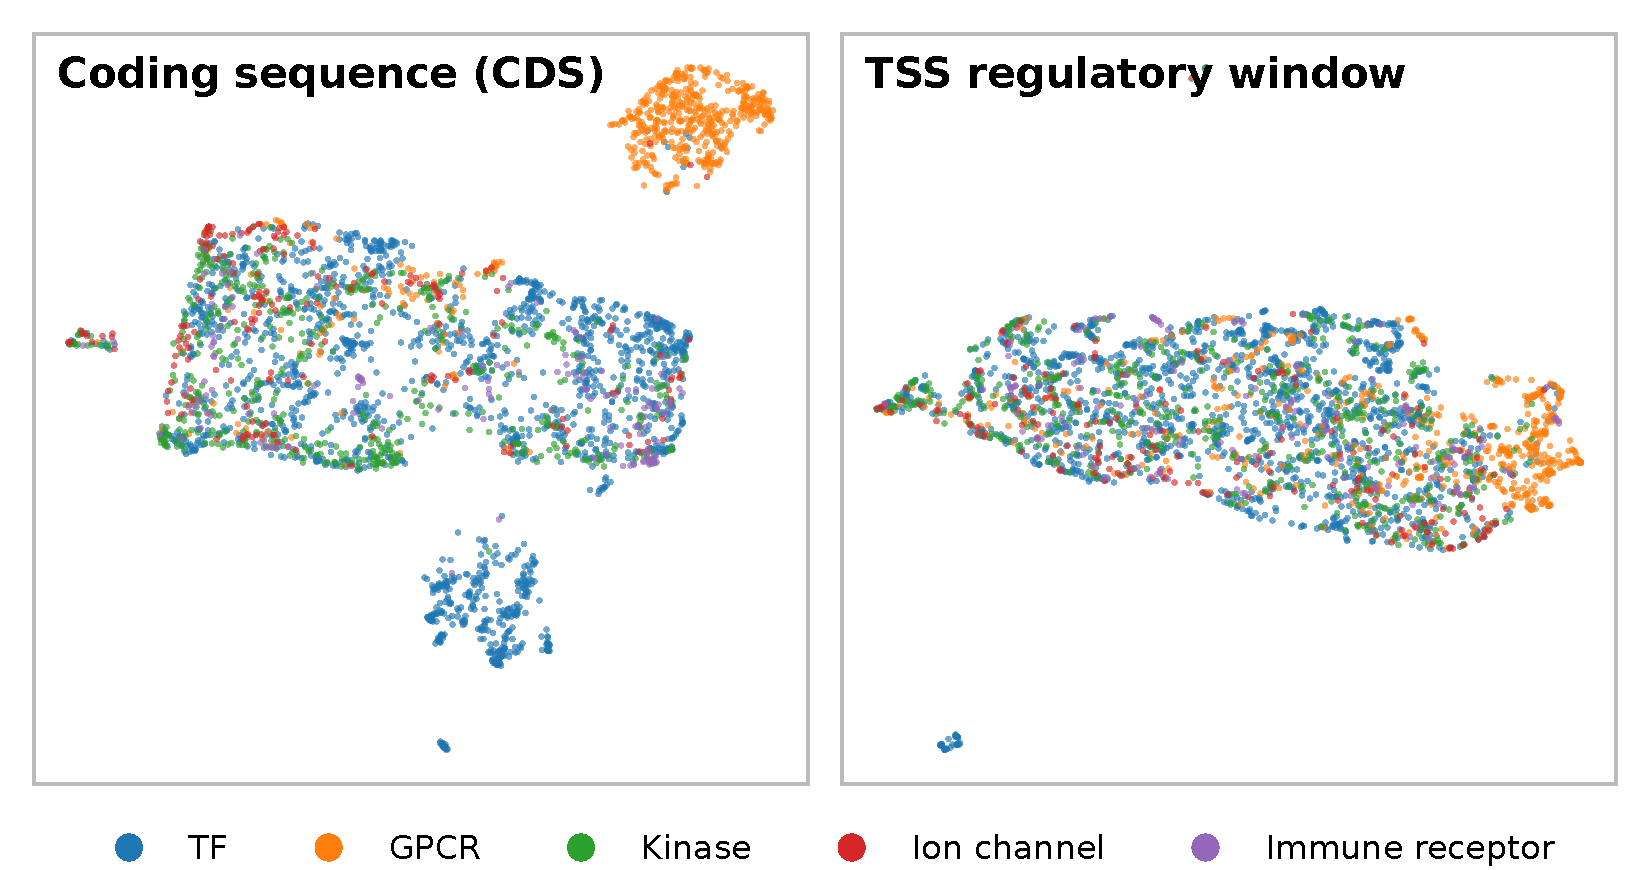
\includegraphics[width=\linewidth]{umap_cds_vs_tss.pdf}\par\vspace{9pt}
    \RaggedRight\Large From a gene's \textbf{coding sequence}, the families separate on
    their own (GPCRs, orange, split off cleanly). Feed the same genes' \textbf{regulatory
    window} and the structure dissolves into one cloud.
  \end{panel}

  \begin{panel}
    \panelhead{\ldots but only up to composition}
    \centering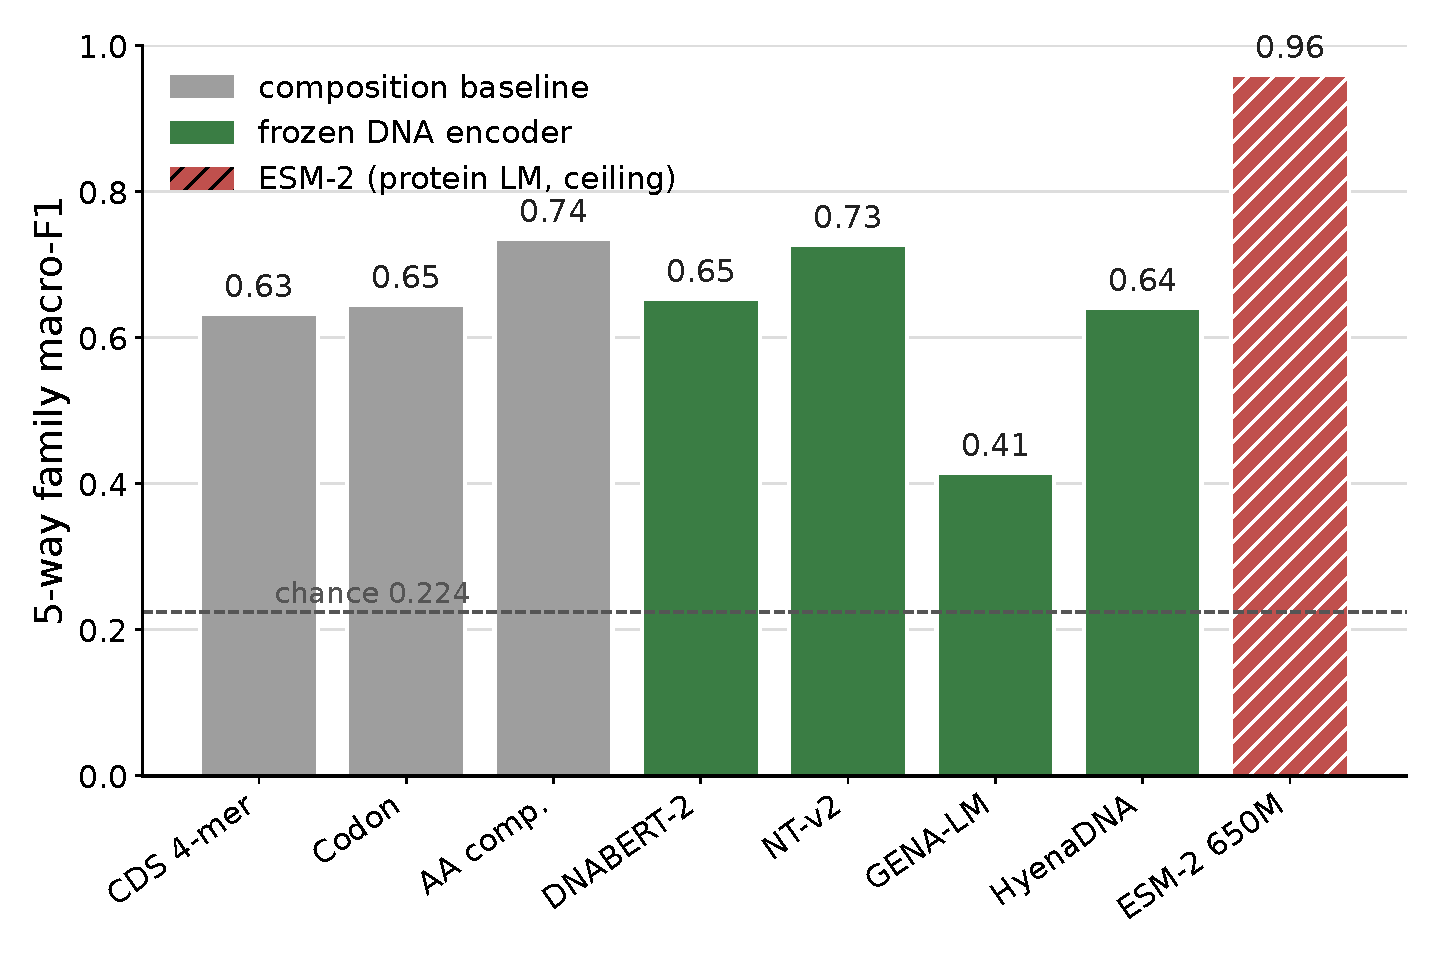
\includegraphics[width=\linewidth]{comparator_f1.pdf}\par\vspace{9pt}
    \RaggedRight\Large The best DNA encoder (NT-v2, \textbf{0.727}) beats simple 4-mer
    composition (0.633) --- but only \emph{ties} translated amino-acid composition
    (0.735), and sits far below a dedicated protein model, ESM-2 (\textbf{0.960}).
    And encoders are \emph{not} interchangeable: GENA-LM (0.415) falls below the baseline.
    \par\vspace{7pt}{\large\color{colBlue}\textbf{Paired test:} vs.\ 4-mer
    $+0.094\,[+0.030,+0.166]$; vs.\ amino-acid composition $-0.008\,[-0.064,+0.056]$,
    a statistical tie.}
  \end{panel}

\end{column}

% ------------------------------ COLUMN 3 ------------------------------
\begin{column}{0.315\paperwidth}

  \begin{panel}
    \panelhead{Regulatory context collapses}
    \centering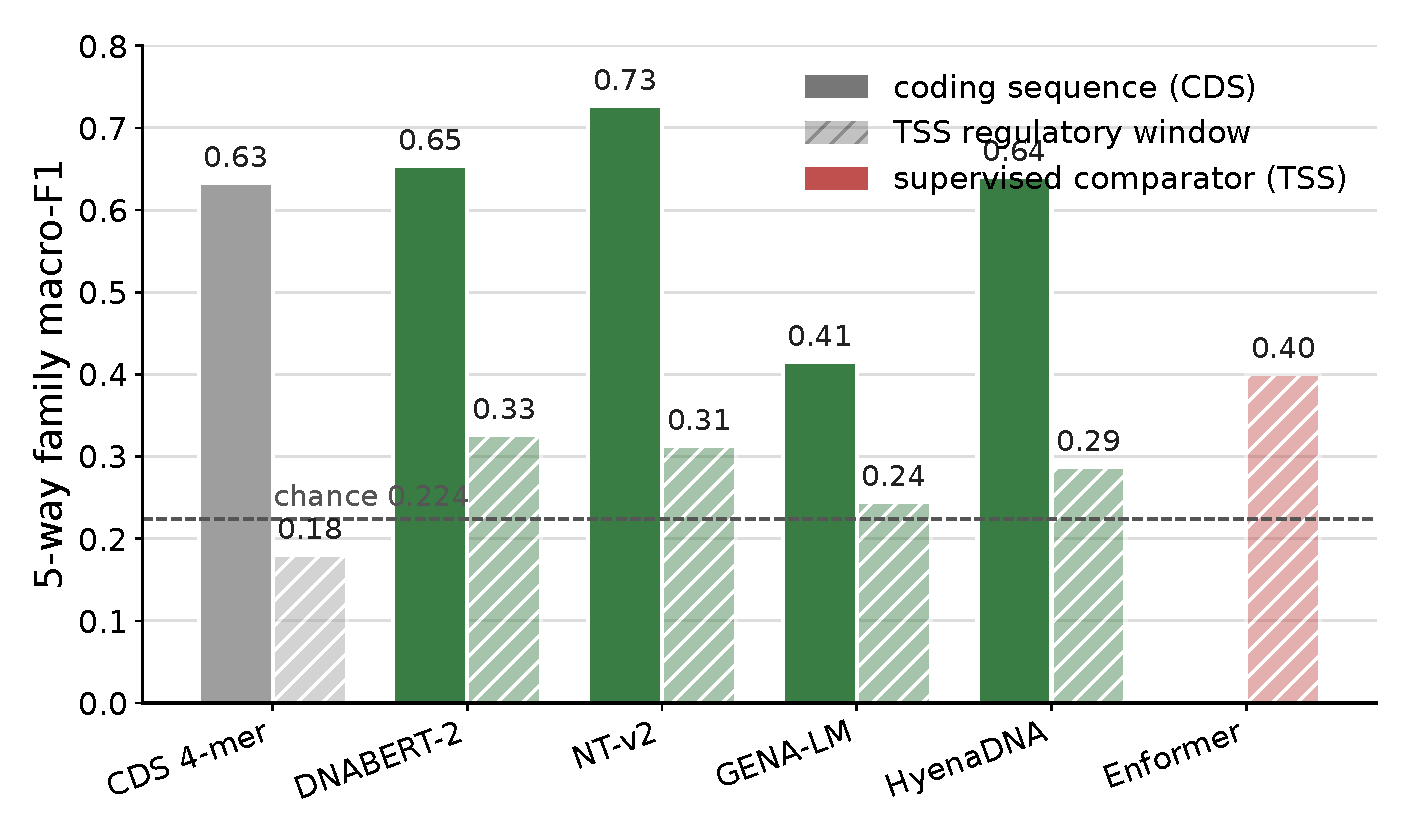
\includegraphics[width=\linewidth]{substrate_collapse.pdf}\par\vspace{9pt}
    \RaggedRight\Large Swap coding sequence for the gene's 196{,}608 bp regulatory (TSS)
    window and family signal falls to near chance (NT-v2 \textbf{0.313} vs.\ 0.224).
    Predicting a gene's natural-language description is weak throughout (best $R^2=0.077$).
    The same collapse holds under a stricter \emph{disjoint}-TSS split
    (NT-v2 $0.313\!\rightarrow\!0.259$).
  \end{panel}

  \begin{panel}
    \panelhead{Honest evaluation matters}
    \centering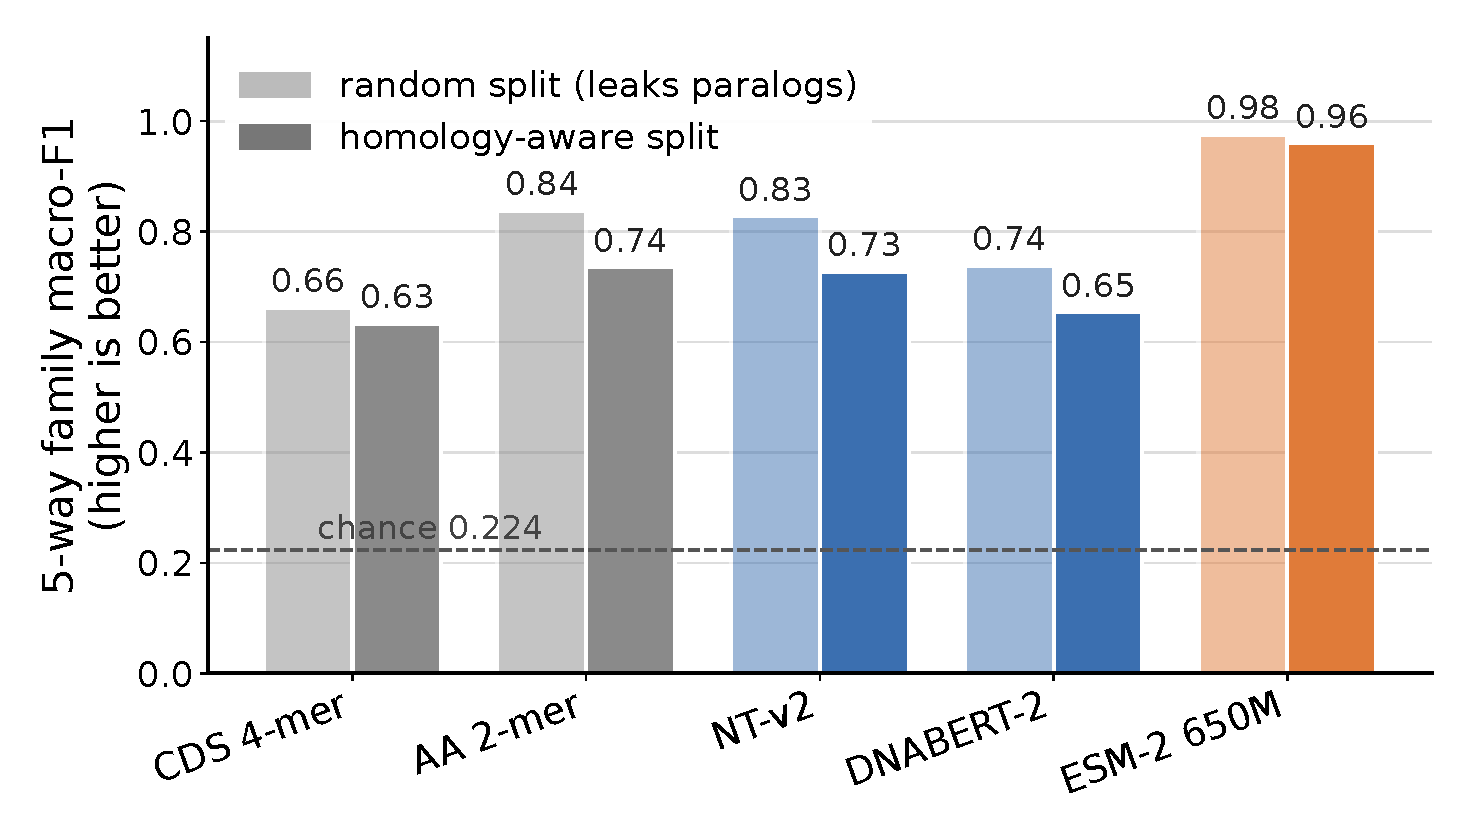
\includegraphics[width=0.82\linewidth]{split_bars.pdf}\par\vspace{6pt}
    \RaggedRight\Large A naive \textbf{random} split inflates every score, because
    near-identical genes leak across train and test. The effect is largest for the
    regulatory arm.
  \end{panel}

\end{column}

\end{columns}

\vspace{10pt}
\begin{takeaway}
  {\color{colBlue}\bfseries\LARGE So what?}\enspace
  \Large Don't treat DNA encoders as generic gene-function models. Trust a benchmark only
  if it has \textbf{(1)} a translated-composition baseline and \textbf{(2)} a homology-aware
  split --- otherwise memorised similarity masquerades as understanding.
  \textbf{MINA is a cheap diagnostic that tells the two apart.}
\end{takeaway}

% =============================== FOOTER ==============================
\vfill
{\color{colAccent!60}\hrule height 1pt}
\vspace{6pt}
{\normalsize\color{cCompos}
 3{,}244 human genes, 5 families \textperiodcentered\ 4 frozen DNA encoders $\times$ 6 poolings
 \textperiodcentered\ homology-aware split (MMseqs2, 40\% identity)
 \textperiodcentered\ macro-F1 with 95\% bootstrap CIs.\hfill
 References: GenePT; ESM-2 (Lin et al.); Nucleotide Transformer; DNABERT-2.\hfill
 Code: github.com/Austin-Senna/dna\_to\_text}

\end{frame}
\end{document}
